\documentclass{beamer}
\usetheme{metropolis}           % Use metropolis theme

%%% Packages
\usepackage{amssymb}
\usepackage{graphicx}
\usepackage{xparse}
\usepackage{multirow}
\graphicspath{ {img/} {../doc/img/} }

\metroset{sectionpage=none}
\metroset{subsectionpage=progressbar}

%fig command. \fig{source}{caption}[optinal width percentage][optional height percentage]
\NewDocumentCommand{\fig}{mmO{1}O{0.8}}
{
	\begin{center}
	\begin{figure}
	  \includegraphics[width=#3\textwidth,height=#4\textheight,keepaspectratio]{#1}
	  \caption*{#2}
	\end{figure}
	\end{center}
}


%%% INFO
\title{Técnicas de aprendizado de máquina para detecção de pessoas em ambiente industrial}
\date{7 de Dezembro de 2016}
\author{Eduardo Henrique Arnold}
\institute{Universidade Federal de Santa Catarina}

%%% Presentation
\begin{document}
	\maketitle

	\section{Introdução}

\subsection{Caracterização da aplicação}
	\begin{frame}{\insertsubsection}
	\fig{wanke3}{Indústria de eletrodomésticos com extrusoras de plástico.}
	\end{frame}

	\begin{frame}{\insertsubsection}
	\fig{wanke2}{Moldes das extrusoras precisam ser substituidos através de uma ponte rolante.}
	\end{frame}

	\begin{frame}{\insertsubsection}
	\fig{wanke1}{Estrutura da ponte rolante pela fábrica.}
	\end{frame}

	\begin{frame}{Sistema de segurança}
		\textbf{Objetivos} \\
		\begin{itemize}
			\item Detectar pessoas automaticamente na região de trabalho.
			\item Impedir movimentação da ponte ao detectar pessoas.
		\end{itemize}

		\pause

		\textbf{Funcionamento} \\
		\begin{itemize}
			\item Câmera de profundidade com vista superior da área de trabalho.
			\item Aprendizado de máquina e visão computacional para detecção de pessoas.
		\end{itemize}
	\end{frame}


\subsection{Métodos de detecção de objetos}
	\begin{frame}{Utilizando descritores}
	\begin{enumerate}
	\item Identificar candidatos.
	\item Utilizar um extrator de características para descrição do objeto.
	\item Introduzir a amostra, proveniente do descritor, em um classificador.
	\end{enumerate}

	\fig{diagram/system}{}[1.1][1]
	\end{frame}

	\begin{frame}{Utilizando aprendizado de representação}
	\begin{enumerate}
	\item Identificar candidatos na imagem.
	\item Introduzir a amostra em um classificador profundo, obtendo a classe correspondente.
	\end{enumerate}

	\fig{diagram/system-deep}{}[1.1][1]
	\end{frame}

	\begin{frame}{Panorama do trabalho}
		\begin{itemize}
			\item Detecção utilizando métodos tradicionais de aprendizado.
			\item Classificação utilizando aprendizado de representação.
			\item Resultados
		\end{itemize}
	\end{frame}

	\chapter{Detecção utilizando métodos tradicionais} \label{chap:tradicional}

O sistema de segurança na fábrica consiste na detecção de pessoas sob a área da ponte. Esse é um problema de localização de objetos, mais especificamente, de detecção de pessoas. Tradicionalmente divide-se essa tarefa em três técnicas de visão computacional: obtenção de candidatos a objeto, obter descrição de cada candidato e então validar a amostra através de classificador. Essa solução foi baseada no trabalho de \cite{rauter}, que propõe um método de obtenção de candidatos e de extração de características. Primeiramente descreve-se aspectos técnicos da aplicação e em seguida cada uma das tarefas para a concretização da solução, por fim, pontos sobre a implementação são mencionados.

\section{Caracterização da aplicação}
Para essa aplicação, recomenda-se a utilização de imagens de profundidade, em que o valor dos pixels indicam a distância entre a câmera e o objeto em questão. Isso se deve ao fato de esse sensor fornecer uma medida independente de luminosidade e variações de cor ou textura se comparada à uma câmera RGB tradicional. Três câmeras foram compradas e avaliadas: \textit{ASUS XtionPRO}, \textit{Orbbec Astra PRO} e \textit{Stereolabs ZED}. As duas primeiras funcionam com o princípio de laser estruturado, já a última funciona baseado em visão estéreo (duas câmeras). Através de testes determinou-se que as maiores distâncias detectadas foram de 4m, 5m e 20m respectivamente. Dado que a câmera será instalada a 6m do chão, em visão superior, optou-se por utilizar a câmera \textit{ZED}.

As imagens recebidas da câmera precisam ser pré-processadas de forma a obter um mapa de distâncias, que é a imagem de profundidade. Isso é feito pela biblioteca fornecida pela \textit{Stereolabs}. Em seguida, inverte-se a imagem (subtrai-se cada pixel da distância da câmera) de maneira que cada pixel forneça a altura em relação ao chão do objeto por ele representado. Além disso pixels cujas distâncias não foram corretamente estimadas são marcados com um valor específico e o resultado é uma imagem cujos valores representam a altura dos objetos em milimetros. Essa informação é relevante pois permite obter candidatos a cabeças de maneira eficiente.

\section{Obtenção de candidatos}
\label{sec:tradicional-candidatos}
O primeiro passo consiste em obter candidatos a pessoas, como a vista é superior, candidatos a cabeças. Em uma aplicação tradicional, com câmeras RGB esse processo dividiria a imagem em pequenos blocos de tamanhos que se espera para uma cabeça, sem qualquer informação sobre o posicionamento, isto é, varrendo uma ``janela imaginária'' pela imagem.

Para aprimorar esse método, assume-se a hipótese de que cabeças serão os objetos mais altos de uma vizinhança, se destacando na cena dos demais objetos. Embora ela não seja sempre verdadeira, ao se verificar que existem máquinas altas, é um método mais eficiente de selecionar candidatos do que utilizar uma janela varrendo todo o quadro.

Aplica-se o método de máximos locais: a imagem é dividida em quadrados de áreas iguais. Para cada quadrado percorre-se os pixels e seleciona-se o maior deles, se este pixel for único no conjunto ele é considerado um ponto candidato à cabeça. Esse processo resulta num conjunto de pontos que determinam candidados à cabeças.

O tamanho dos quadrados que dividem a imagem é fundamental nessa etapa: se forem muito grandes há alta probabilidade de se perder cabeças visto que na cena existem máquinas altas. Por outro lado, se forem muito pequenos, existirão muitos candidatos e o processo se torna lento. Esse tamanho é calculado \cite{rauter} utilizando a equação 
\begin{equation}
	\label{eq:cam-proj}
	s_w = \frac{f}{d} \cdot s_r
\end{equation}
 onde $f$ é a distância focal da câmera, a $d$ a distância média entre a câmera e as pessoas e o $s_r$ o tamanho padrão de cabeças.

Em seguida, é necessário determinar um quadrado que delimite a cabeça de forma centralizada. Para obter o tamanho do quadrado, novamente utiliza-se a equação \eqref{eq:cam-proj}, porém dessa vez utilizando o valor do pixel encontrado para aquele candidato como altura. Tem-se então um quadrado de tamanho apropriado com o pixel máximo no centro, porém em poucos casos esse quadrado centraliza a cabeça.

Utiliza-se um processo de centralização baseado em \textit{mean shift}, que permite iterativamente localizar o máximo de uma função probabilidade dado uma máscara. Nesse caso, uma interpretação do procedimento é mover o quadrado mantendo suas dimensões fixas para o centróide dos pixels que estão em seu interior. Intuitivamente, percebe-se que os pixels de valor mais elevado terão maior peso, portanto, espera-se que o quadrado seja centralizado sob parte central da cabeça.

Atualiza-se o centro do retângulo
\begin{equation}
	\label{eq:mean-shift}
	m(p) = \frac{\sum_{p_i \in S(p)} I(p_i)p_i}{\sum_{p_i \in S(p)} I(p_i)}
\end{equation}
onde $I$ é a imagem e $S(p)$ é o conjunto dos pixels no quadrado de centro $p$.

\begin{figure}[h]
\centering
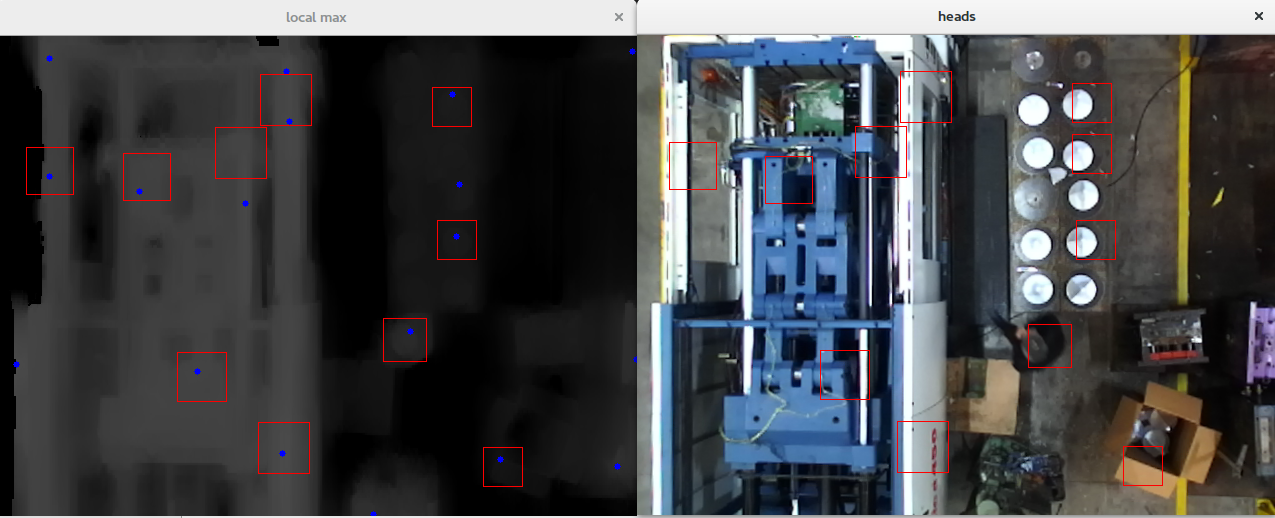
\includegraphics[width=0.8\textwidth]{tradicional/candidatos}
\caption{Pontos em azul são máximos locais e os quadrados vermelhos indicam os candidatos centralizados}
\label{fig:candidatos}
\end{figure}

Ao final dessa etapa, conta-se com uma lista de candidatos representados pelo \textit{patch} da imagem correspondente, como ilustrado na Figura \ref{fig:candidatos} pelos quadrados em vermelho.

\section{Descritores}
\label{sec:tradicional-descritores}
Tendo a lista de candidatos é necessário obter uma descrição para cada um deles. No trabalho de referência \cite{rauter} se destacam dois descritores: grades simples e grades circulares. Um terceiro descritor é proposto no presente trabalho para substituir o de grades circulares. Observa-se que para todos os descritores a característica importante de representação está nos desníveis da cabeça em relação ao resto do corpo, que se dá de maneira aproximadamente circular. Portanto, objetiva-se encontrar uma maneira de evidenciar quando e em que grau esse tipo de padrão ocorre.

O primeiro descritor, grades simples, divide o candidato em blocos, com uma quantidade ímpar em cada dimensão, como ilustrado na Figura \ref{fig:descritores}. Para esse descritor em específico, fixou-se a quantidade de blocos em 7 para cada dimensão com 49 blocos no total, pois avaliou-se que para o tamanho dos candidatos esta foi a representação mais adequada. Então calcula-se a média dos pixels em cada um dos blocos, gerando uma matriz de médias 7x7. Em seguida, subtrai-se dessa matriz o valor da média do bloco central. Por fim, gera-se um histograma da matriz resultante com número de intervalos igual a 32. Esse vetor de histograma é considerado o vetor de descrição (\textit{feature vector}), cuja soma é 49.

Já o segundo método, grades circulares, apresentado em \cite{rauter}, propõe que uma série de blocos quadrados seja disposta circularmente sobre a imagem candidata e que o mesmo procedimento do primeiro extrator seja realizado. O objetivo seria ter um descritor com maior invariância à rotação, dada a distribuição dos blocos. Porém, esse extrator é difícil de implementar devido à variação do tamanho dos candidatos.

Para facilitar a implementação, propomos, então, um descritor de anéis concêntricos. A ideia é similar às grades circulares, porém ao invés de se dispor blocos de maneira circular, utilizam-se coroas que partem desde o centro da imagem até as bordas. Primeiramente divide-se a imagem em $n$ coroas circulares cujo centro coincide com o da imagem e cuja diferença entre os raios é constante, como visto na Figura \ref{fig:descritores}. Então gera-se um vetor $v \in \RR^n$ em que cada elemento corresponde à média dos pixels pertencentes à $n$-ésima coroa, desconsiderando os pixels inválidos. Em seguida subtrai-se desse vetor o valor da média da primeira coroa, cujo raio menor é 0 correspondendo então à um círculo. Por fim a descrição do candidato corresponde à diferenciação discreta (diferenças entre as componentes adjacentes) desse vetor, para evidenciar ainda mais as diferenças entre as alturas médias das coroas. Note que o vetor de descrição tem dimensão $d=n-1$. Para esse descritor diferentes valores de $n$ foram avaliados para identificar a melhor divisão, conforme descrito no Capítulo \ref{chap-resultados}.

Após obter a descrição de cada candidato é possível classificá-los de maneira a validar que são cabeças de fato.

\begin{figure}[h]
\centering
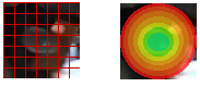
\includegraphics[width=0.8\textwidth]{tradicional/descritores}
\caption{Ilustração dos descritores: grades simples e anéis concêntricos.}
\label{fig:descritores}
\end{figure}

\section{Classificação}
\label{sec:classificacao:svm}
%Referência SVM http://www.cs.columbia.edu/~kathy/cs4701/documents/jason_svm_tutorial.pdf

Utiliza-se um classificador binário SVM (\textit{Support Vector Machine}). Seja o dataset o conjunto $(x_i, y_i)$ para $i=1 \dots N$ com $x_i \in \RR^d$ sendo o vetor de descrição do candidato $i$ e $y_i \in \{-1, 1\}$ sendo a classe correspondente, não-cabeça ou cabeça, respectivamente. Deseja-se encontrar um classificador $f(x)$ tal que 
\begin{equation*}
\label{eq:svm-decision}
	\begin{cases}
		f(x_i)>0,& \text{se } y_i=1 \\
		f(x_i)<0,& \text{se } y_i=-1 \\
	\end{cases}
\end{equation*}
 ou seja, $y_i f(x_i) > 0$ para uma classificação correta. 

A função de decisão do SVM pode ser descrita como $f(x)=w^T x+ b$ onde $w \in \RR^d$ é o vetor de pesos, que fornece a inclinação do hiperplano e $b \in \RR$ um deslocamento do hiperplano em relação à origem. Define-se ainda a margem como a menor distância entre o hiperplano de separação e qualquer amostra, dada por $\frac{2}{\|w\|}$ onde
\begin{equation}
\|w\| = \sqrt{w_1^2 + \dots + w_n^2}.
\end{equation}

O aprendizado consiste em encontrar $w$ e $b$ que maximizem a a margem sujeitos à $y_i(w^T x_i+b) \geq 1$. Esse é um problema de otimização convexa, em que qualquer mínimo local é também global. Assim, minimiza-se a função custo \cite{bishop2007}
\begin{equation}
	\label{eq:svm-cost}
	\min P(w,b) = \frac{1}{2}\|w\|^2 + C\sum_i H_1(y_i f(x_i)).
\end{equation}
onde a função
\begin{equation*}
H_1(z)=\max(0,1-z)
\end{equation*}
é utilizada para dar um peso negativo quanto maior for o erro do classificador (quando o argumento é negativo).

O primeiro termo da equação \eqref{eq:svm-cost} está associado à maximização da margem e o segundo à minimização dos erros de treinamento, quando uma amostra é classificada erroneamente. O parâmetro $C$ controla quanto se penaliza os erros de classificação diante da maximização da margem, visto existir uma relação ideal entre eles.

O dataset é considerado linearmente separável se for possível encontrar uma reta ou hiperplano que separe todas as amostras corretamente. Entretanto nem sempre que for linearmente separável a classificação sem erros é o ideal. Por exemplo, o dataset apresentado Figura \ref{fig:svm-margin} mostra que optar pela separação ótima gera perda de generalização. Fica evidente que nesse caso deveria-se priorizar uma margem maior em detrimento de alguns possíveis erros de classificação, o que pode ser feito diminuindo o valor de $C$.

\begin{figure}
\centering
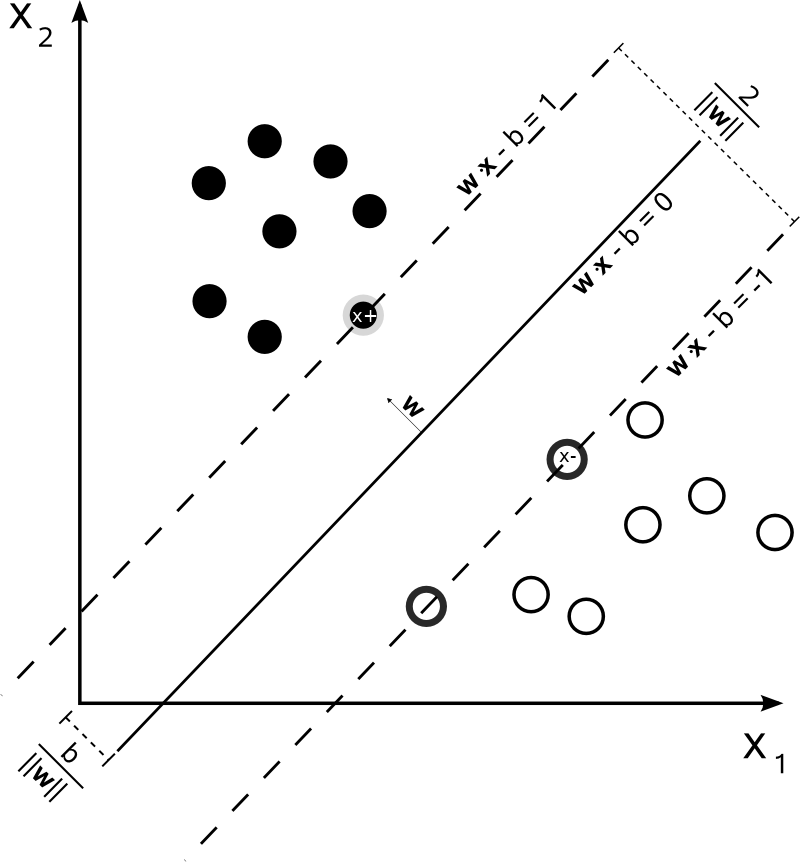
\includegraphics[width=0.3\textwidth]{svm/svm-margin}
\caption{Exemplos de dataset em que separação perfeita não é ideal}
\label{fig:svm-margin}
\end{figure}

O modelo de SVM apresentado até aqui é conhecido como linear. Mesmo com o método de penalização de erros de classificação, datasets complexos podem não ter um desempenho satisfatório. Dessa maneira, é introduzido um modelo não linear para o classificador: transforma-se as amostras $x_i$ em um novo espaço obtendo amostras $\Phi(x_i)$ que são, no caso ideal, linearmente separáveis, como mostrado na Figura \ref{fig:svm-kernel}.

\begin{figure}
\centering
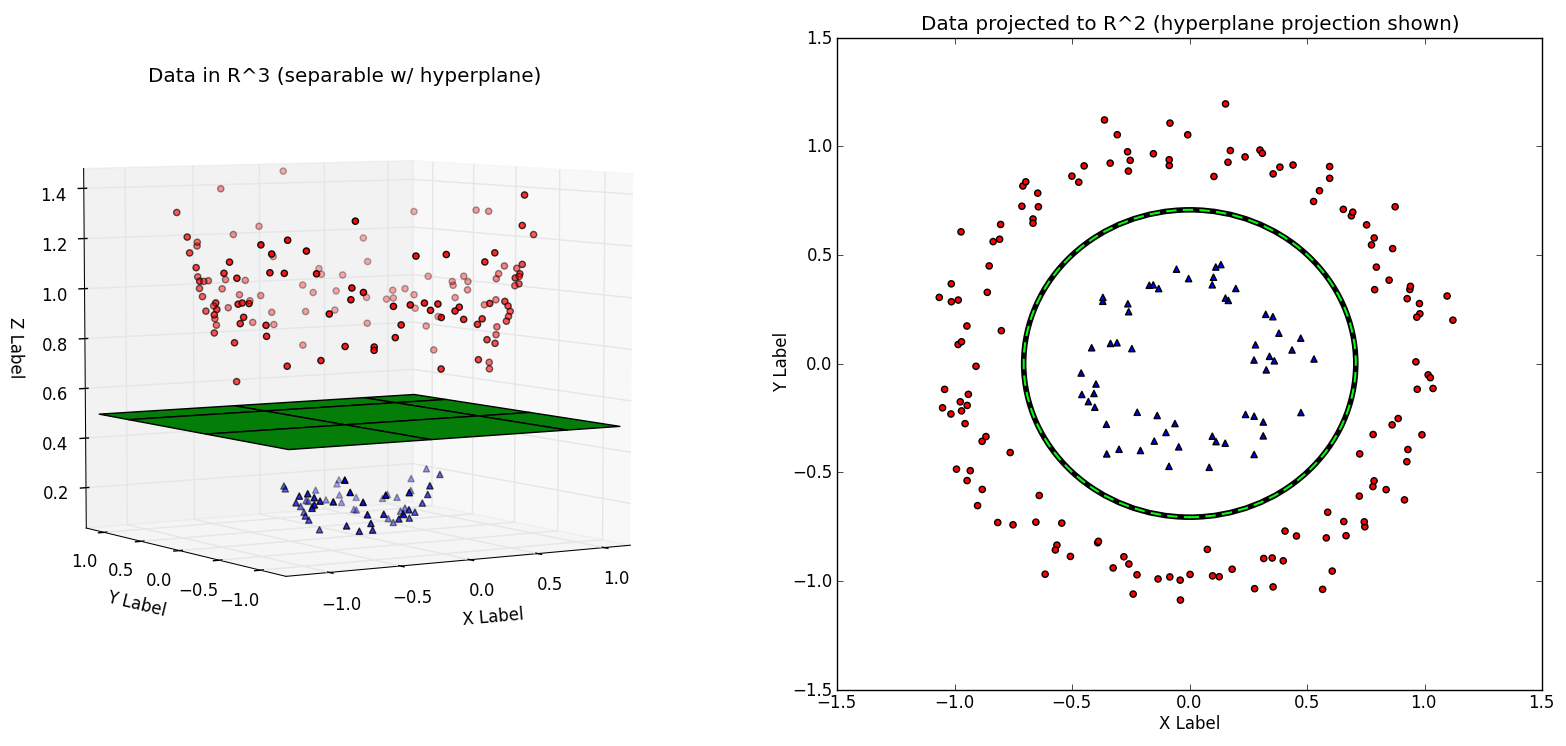
\includegraphics[width=0.8\textwidth]{svm/svm-kernel}
\caption{Exemplo de mapeamento para obter um classes linearmente separáveis. Espaço transformado e original, respectivamente.}
\label{fig:svm-kernel}
\end{figure}

Formalmente \cite{bishop2007} tem-se a função decisão modificada como
\begin{equation*}
f(x)=w^T \Phi(x) +b.
\end{equation*}
Na prática, entretanto, não se calcula as coordenadas da amostra transformada no novo espaço. Ao invés disso utiliza-se o chamado \textit{kernel trick} \cite{bishop2007} em que o produto interno entre duas amostras transformadas é obtido diretamente através da avaliação da função $\Phi(x)$ sob as amostras originais.

Segue do teorema da representação de Kimeldorf e Wahba \cite{kimeldorf1970correspondence} que
\begin{equation}
	\label{eq:teo-kimeldorf}
	w=\sum_{i=1}^m \alpha_i \Phi(x_i)
\end{equation}
para alguma variável $\alpha$. Portanto, ao invés de minimizar $w$ diretamente, podemos minimizar $\alpha$ e a função decisão se torna
\begin{equation}
	\label{eq:svm-decision-func}
	f(x)=\sum_{i=1}^m \alpha_i \Phi(x_i) \Phi(x) +b.
\end{equation}

Chamamos $K(x_i, x) = \Phi(x_i) \cdot \Phi(x)$ de \textit{kernel} ou função núcleo. Um exemplo bastante utilizado é a \textit{Radial Basis Function} (RBF), também conhecida como núcleo gaussiano, dada por
\begin{equation}
	\label{eq:svm-kernel-func}
	K(x,x_i) = \exp\left(-\frac{\|x-x_i\|^2}{2\sigma^2}\right).
\end{equation}
Nota-se que quando $\|x-x_i\|$ é muito maior que $\sigma$ a função retorna um valor que tende a zero, o que demonstra que a amostra em questão tem pouca importância para o hiperplano de decisão. Assim, quanto menor o valor de $\sigma$, mais local tende a ser o classificador, o que faz com que o desempenho no conjunto de treinamento seja excelente. Porém, ao mesmo tempo proporciona menor generalização do modelo, o que significa que esse desempenho não se replica no conjunto de teste.

\section{Variação para saída probabilística}
\label{sec:svm-probabilistic}
A formulação tradicional do SVM possui saída categórica, isto é, a classe à qual a amostra pertence. Entretanto, para uma classificação binária, é possível adicionar um componente que permite estimar uma saída probabilística, isto é, a probabilidade da amostra ser positiva.

A função de decisão \eqref{eq:svm-decision} é proporcional à distância (com sinal) da amostra até o hiperplano de separação. Redimensionando essa medida através da função de Platt \cite{svmProbabilisticOutput} é possível obter a probabilidade da amostra pertencer à determinada classe $P(y_i=1 | x_i)$. A função de Platt é simplesmente uma regressão logística, cujos parâmetros são encontrados por otimização após o treino do SVM tradicional. Permitindo, então, obter uma saída probabilística de um classificador SVM.

Essa formulação é interessante pois dá flexibilidade do rigor da classificação através da escolha do limiar de probabilidade a partir do qual uma amostra é considerada positiva após o modelo ter sido treinado.

\section{Implementação}
Para os algoritmos de processamento de imagens e extração de características, fez-se uso da biblioteca \textit{OpenCV} que implementa grande quantidade de operações básicas em imagens e fornece um ambiente rico de trabalho para criar novas funcionalidades.

No que se refere a aprendizado de máquina, utilizou-se a biblioteca \textit{Scikit-learn} \cite{scikit-learn} que implementa o algoritmo de treinamento SVM. Além de fornecer as amostras, no caso, a descrição dos candidatos, é necessário configurar os parâmetros $C$, para penalidade dos erros de treinamento e o parâmetro $\sigma$ do \textit{kernel RBF}. 

A abordagem utilizada foi o método de treinamento automático fornecido pela biblioteca: indica-se um conjunto de elementos para cada um dos parâmetros e todas as combinações de parâmetros são testadas utilizando um processo de validação cruzada. Basicamente divide-se o conjunto de treinamento em 5 conjuntos dos quais quatro são utilizados para treinamento e um para validação. Ao final do procedimento as estatísticas de cada tentativa é exibida e a que tiver melhor desempenho, segundo métrica estabelecida, é escolhida. Tendo obtido esses parâmetros um novo processo de treinamento é efetuado, agora utilizando todo o conjunto de treinamento, sem validação.

Nota-se ainda que é possível utilizar de todos os núcleos do processador com essa biblioteca, o que traz um impacto bastante positivo na performance temporal do algoritmo.

Tendo treinado o modelo é possível obter o resultado da classificação para cada candidato e remover os que não forem reconhecidos como cabeças. O resultado final do processo é um vetor de quadrados contendo todas as cabeças encontradas no quadro.

	%\chapter{Classificação utilizando aprendizado profundo}

O capítulo anterior tratou-se de uma solução baseada em seleção de candidatos, extração de características e posterior classificação, o que caracteriza uma técnica superficial. Nesse capítulo propomos uma solução híbrida, que utiliza a seleção de candidatos idêntica à anterior, porém utiliza técnicas profundas de classificação de modo que os candidatos são diretamente inseridos no classificador. Inicialmente introduz-se as redes MLP e convolucionais, fornecendo as bases teóricas, funções de ativação e processo treinamento.  Questões relativas à implementação também são abordadas.

\section{Perceptron Multicamadas (MLP)}

Segundo \cite{DLbook}, uma rede de perceptrons multicamadas (MLP) também pode ser chamada de rede profunda sem realimentação (\textit{deep feedforward networks}), um exemplo de rede neural, e tem como objetivo aproximar uma função $f*$. Para o problema de classificação, $y=f*(x)$, onde $y$ é a categoria e $x$ a amostra, a rede define um mapeamento $y = f(x,\theta)$, onde $\theta$ são os parâmetros do modelo. O problema consiste em encontrar $\theta$ que resulte na melhor aproximação de $f^*$.

Essa estrutura é chamada de rede pois são representadas como um conjunto de camadas, cada uma alimentando a próxima, o que gera uma cadeia de funções: $y=f^1(f^2(f^3(x)))$, cada qual representando uma camada. Além disso, não ocorre alimentação pois a informação flui continuamente através das camadas desde a entrada $x$ sequencialmente até a camada de saída $y$.

Parte-se de um modelo linear simples,
\begin{equation}
y=x^Tw
\end{equation}
em que $w$ corresponde ao vetor de pesos do classificador. Verifica-se que esse modelo pode ser treinado de maneira simples e rápida, porém serve apenas para casos em que o dataset é linearmente separável, diferente da maioria dos problemas reais. Como visto na seção \ref{sec:classificacao:svm}, técnicas de mapeamento não lineares $\phi(x)$ são alternativas para tentar tornar essas amostras linearmente separáveis, como é o caso da função RBF. Na abordagem superficial de classificação, deve-se escolher esse mapeamento de maneira específica às amostras de forma manual. 

Advém, então, uma das principais contribuições dos métodos profundos: a função de mapeamento $\phi(x,\theta)$ é determinada, entre uma gama ampla de funções, pelo próprio sistema através dos parâmetros $\theta$. Isso pode ser interpretado como a seleção automática, pelo algoritmo, do extrator de características que melhor represente o dataset. Assim, o modelo se torna 
\begin{equation}
y=f(x,\theta,w) = \phi(x,\theta)^Tw
\end{equation}
Na rede, $\phi$ corresponde à camada intermediária. Os parâmetros $w$ mapeiam, então, o resultado da camada intermediária $\phi(x,\theta)$, que representam as descrições da amostra, para a camada de saída $y$. O princípio de aprender o extrator características mais apropriado para o dataset não é exclusivo para redes MLP e se aplica a outros modelos de aprendizado profundo.

\section{Funções de ativação}
Como visto na seção \ref{introducao:perceptron}, os perceptrons aplicam uma função de ativação ao somatório ponderado das entradas. A escolha dessa função está associada à interpretação que se dá à saída. Além disso é fundamental que as funções de ativação sejam compatíveis com a função custo para evitar problemas como o gradiente enfraquecido, como será visto adiante. Duas funções foram utilizadas nesse trabalho e serão introduzidas a seguir.

\subsection{Sigmoide}
Como visto anteriormente, a escolha da função relaciona-se com a interpretação do valor de saída. Para classificadores interpreta-se o valor dos perceptrons da camada de saída como probabilidades da amostra pertencer a uma determinada classe. Nesse caso espera-se que esses valores estejam no intervalo $[0,1]$. Uma função que assegura essa condição é a sigmoide
\begin{equation}
	\label{eq:sigm}
	\sigma(x) = \frac{1}{1+e^{-x}}
\end{equation}

\begin{figure}[h]
\centering
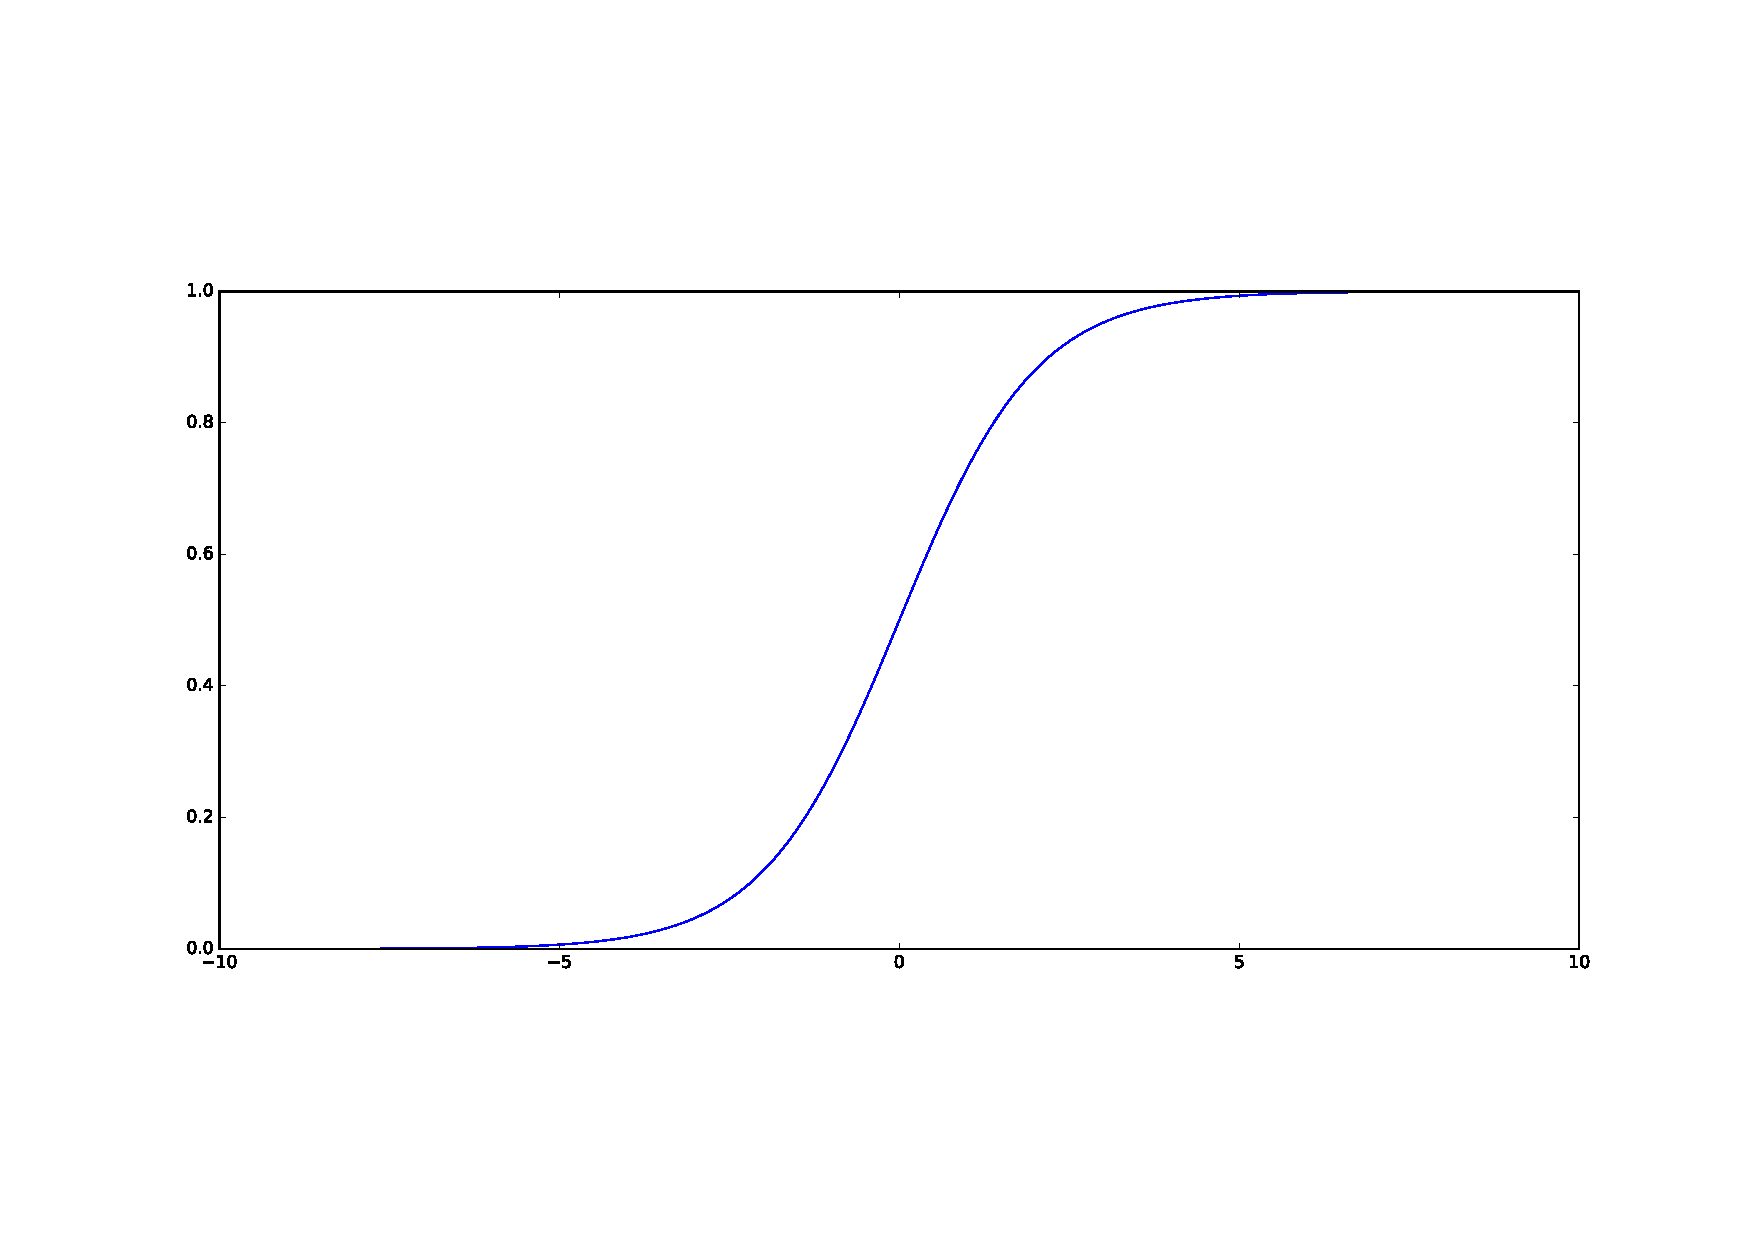
\includegraphics[width=0.9\textwidth]{deep/sigmoid}
\caption{Gráfico mostrando o comportamento da sigmoide}
\label{fig:sigmoid}
\end{figure}

Outra característica importante é a não linearidade da função que permite transformar conjuntos não linearmente separáveis. Por outro lado, observa-se que essa função satura facilmente com entradas de alta amplitude, ocasionando uma derivada praticamente nula nessas regiões. Como será visto adiante isso é um problema ao se considerar que a derivada dessa função definirá a atualização dos pesos desses perceptrons durante o processo de treinamento. Portanto, uma derivada pequena significa que o perceptron demorará a ter seus pesos atualizados. Ao propagar esse processo camada a camada, verificam-se derivadas cada vez menores, o que causa o problema do gradiente enfraquecido, em que as camadas iniciais não conseguem aprender pois o gradiente é muito reduzido.

\subsection{RELU}
Para resolver o problema do gradiente enfraquecido a \textit{Rectified Linear Unit -- RELU} foi proposta \cite{nair2010relu} como
\begin{equation}
	\label{eq:relu}
	\text{RELU}(x) = \max(0,x)
\end{equation}

Observa-se que para valores positivos essa função tem uma derivada constante e igual a um, proporcionando uma taxa de aprendizado considerável sempre que o perceptron estiver ativo. Por outro lado, para valores negativos considera-se o perceptron inativo e os pesos não são atualizados. Ao mesmo tempo essa característica garante a não linearidade da função.

\section{Treinamento}
O processo de treinamento de uma rede neural é um problema de otimização. Porém, diferentemente do caso do SVM, trata-se de uma otimização não convexa, isto é, existem múltiplos mínimos locais para a função custo e diversas soluções podem ser encontradas, dependendo dos valores iniciais dos parâmtros. Esse fato advém do caráter não linear das funções de ativação nas camadas intermediárias que irão definir a extração de características.

Durante essa etapa otimiza-se os parâmetros $\theta$ de forma que $y \approx f*(x)$. Isso é feito através da minimização de uma função custo, que mede a proximidade entre os resultados do modelo e o conjunto de treinamento. Em geral escolhe-se a função de entropia cruzada
\begin{equation}
J(\theta) = -\log P(y|x)
\end{equation}
A escolha da função custo está associada também à função de ativação das camadas de saída. Isso é importante pois no caso de uma ativação sigmoide a saída satura rapidamente, o que provoca uma derivada muito pequena que ocasionará um gradiente pequeno e consequentemente 

Observa-se que a camada de saída possui um valor alvo bem definido, porém as camadas intermediárias (\textit{hidden layers}) não têm um comportamento diretamente especificado. Nesse caso, utiliza-se o algoritmo de propagação reversa de erros (\textit{back-propagation}).


\section{Redes convolucionais}

\section{Implementação}
Keras e theano. Diferentes configurações.

	\chapter{Resultados}
Nesse capítulo os resultados das diferentes soluções propostas no trabalho são apresentados. Primeiramente introduzem-se as medidas de avaliação que serão utilizadas. Em seguida compara-se as etapas de classificação do método tradicional e híbrido, cujo processo de seleção de candidatos é idêntico, portanto a diferença em desempenho se dá apenas no estágio de classificação. Por fim avalia-se o desempenho do sistema completo das diferentes soluções apresentadas.

\section{Medidas de avaliação}
Para avaliar o desempenho das diferentes soluções apresentadas nesse trabalho se faz necessário a utilização de medidas que permitam comparar os resultados objetivamente e indicar facilmente os aspectos positivos e negativos relevantes de cada método. Nesse trabalho tratamos de classificação binária, em que amostras são positivas (representando cabeças e também indicadas por 1) ou negativas (representando não-cabeças e também indicadas por 0). 

Em geral, num problema de classificação o indicador mais comum é a acurácia (\textit{accuracy}), definida \cite{evaluationMetrics} como a razão das classificações corretas pelo total de classificações. É fundamental notar, entretanto, que essa medida sozinha não é suficiente para avaliar um classificador, especialmente se o dataset for desbalanceado. Por exemplo, ao considerar um dataset com duas amostras negativas entre 20 e utilizar um classificador trivial que classifica qualquer amostra como sendo positiva, obtem-se uma acurácia de 90\%, demonstrando o problema dessa métrica.

Uma maneira compacta de representar o desempenho de um classificador é a \textbf{matriz de confusão} \cite{evaluationMetrics}, apresentada na tabela \ref{tab:matriz-confusão}. Para uma classificação binária é uma matriz 2x2 em que a primeira linha indica as amostras negativas e a segunda as amostras positivas. De forma semelhante, a primeira coluna indica amostras que foram classificadas como negativas e a segunda que foram classificadas como positivas. Combinando-se essas linhas e colunas, obtém-se o número de verdadeiros negativos TN, falsos positivos FP, falsos negativos FN e verdadeiros positivos TP, respectivamente. Essa estrutura supera os problemas da acurácia pois fornece a distribuição de acertos e erros de classificação. Adota-se a descrição dos valores em percentuais relativos ao conjunto de análise.

\begin{table}
\centering
\caption{Matriz de confusão}
\label{tab:matriz-confusão}
\begin{tabular}{ll|l|l|}
\cline{3-4}
                                            &   & \multicolumn{2}{l|}{Classificado} \\ \cline{3-4} 
                                            &   & 0               & 1               \\ \hline
\multicolumn{1}{|l|}{\multirow{2}{*}{Real}} & 0 & \text{TN}              & \text{FP}              \\ \cline{2-4} 
\multicolumn{1}{|l|}{}                      & 1 & \text{FN}              & \text{TP}              \\ \hline
\end{tabular}
\end{table}

Outro aspecto a destacar na avaliação de classificadores é que não basta avaliar os indicadores apresentados apenas no conjunto de treinamento. Embora essas medidas forneçam um limite máximo para o desempenho do classificador e permitam detectar \textit{underfitting}, quando o modelo não tem capacidade de modelar o conjunto de treinamento, não se pode avaliar o desempenho do classificador em um caso geral, isto é, não incluso no conjunto de treinamento. Por outro lado, se o modelo for demasiadamente complexo ele pode ter se tornado muito específico para algumas características do conjunto de treinamento, situação conhecida como \textit{overfitting}. Assim, para medir o desempenho do classificador em uma situação real utiliza-se de outro conjunto de dados supervisionados chamado de conjunto de teste (\textit{test set}), independente do conjunto de treinamento. Afirma-se que o modelo generaliza bem se o desempenho no conjunto de treinamento se equiparar ao de teste.

Graficamente pode-se avaliar classificadores através do gráfico ROC (\textit{Receiver Operating Characteristic}) \cite{evaluationMetrics}, que relaciona a taxa de verdadeiros positivos
\begin{equation}
\text{TVP} = \frac{\text{TP}}{\text{FN}+\text{TP}}
\end{equation}
com a taxa de falsos positivos 
\begin{equation}
\text{TFP} = \frac{\text{FP}}{\text{TN}+\text{FP}}.
\end{equation} 
Dessa forma, o classificador ideal indicaria uma TVP unitária com TFP nula, o que caracteriza o ponto $(0,1)$.

A princípio cada classificador avaliado em um conjunto de dados corresponde a um ponto no espaço ROC. Entretanto existem classificadores cuja saída é a probabilidade da amostra ser positiva. Nesses casos é possível escolher um limiar de probabilidade $T$ acima do qual se considera uma amostra como positiva. Cada escolha desse limiar corresponderá a um ponto no espaço ROC e variando esse parâmetro é possível obter uma curva nesse espaço.

Comparar diferentes classificadores não é trivial pois é uma tarefa multiobjetivo que envolve simultaneamente maximizar a TVP e minimizar TFP. Portanto só é possível afirmar que um classificador é melhor do que outro sse sua TVP é maior e sua TFP é menor que a do outro, nesse caso diz-se que o primeiro domina o segundo. Na prática, entretanto, pode-se utilizar a métrica \textit{Area Under Curve}, AUC, que mede a área sob a curva ROC, para facilitar essa comparação, especialmente quando a região de operação não é especificada.

Um requerimento específico para a aplicação em questão é que a linha de produção se mantenha em funcionamento o maior tempo possível, para tanto deve-se minimizar a quantidade de falsos positivos FP, que significam cabeças incorretamente identificadas que interrompam a produção sem necessidade. Assim, demanda-se uma TFP menor que 10\%. Quando especificada, a AUC será correspondente à área sob a curva ROC com TFP inferior à esse limite.

\section{Desempenho dos Classificadores}
\label{sec:resultados-classificadores}
O classificador SVM originalmente possui saída categórica, porém pode ser adaptado para fornecer uma saída probabilística que indica a probabilidade da amostra ser positiva conforme visto na seção \ref{sec:svm-probabilistic}. Nota-se entretanto que internamente a formulação é ainda categórica. Já os métodos profundos possuem saídas probabilísticas por definição. Essa estrutura da saída como probabilidade é vantajosa pois permite ajustar o compromisso entre falso positivos e falso negativos do classificador, após treinamento, através da escolha do limiar de probabilidade $T$ acima do qual uma amostra é considerada positiva. Escolher um limiar mais alto significa exigir mais segurança do classificador e, portanto, reduzir o número de falsos positivos ao preço de aumentar o número de falsos negativos.

No caso de saídas probabilísticas, para representar a matriz de confusão se faz necessário escolher valores para $T$. Nesse trabalho escolhem-se dois valores (0.5 e 0.9) para esse parâmetro de maneira a demonstrar sua influência sob a distribuição das amostras na classificação. Nota-se que a estrutura de classificação é a mesma, apenas o limiar é trocado.

Para realizar o treinamento dos classificadores foi gerado um conjunto de dados a partir de gravações realizadas no ambiente indústrial onde o sistema deverá ser instalado. A câmera foi posicionada num ponto próximo de onde deve ocorrer a sua instalação final. Diversos vídeos foram gravados e posteriormente analisados. Utilizando o algoritmo de detecção de candidatos visto em \ref{sec:tradicional-candidatos}, selecionou-se manualmente em cada quadro quais dos candidatos eram verdadeiramente cabeças.

Repetindo esse processo em cada quadro formou-se um conjunto de treinamento, cuja amostra é o recorte do candidato, reduzido de 2459 amostras negativas (não cabeças) e 667 positivas (cabeças). Em seguida estendeu-se esse conjunto reduzido para 9894 amostras negativas e 1222 positivas, formando o conjunto de treinamento completo. Para averiguar o desempenho estendeu-se esse conjunto para 16898 amostras das quais 14966 são negativas. Criou-se, ainda, um conjunto de teste independente de 2738 amostras negativas e 235 amostras positivas.

\subsection{SVM}
Avaliou-se o resultado dos diferentes descritores mencionados em \ref{sec:tradicional-descritores} utilizando um processo de treinamento automático do SVM \cite{scikit-learn}: varreu-se o espaço dos parâmetros $C$ entre $0.0001$ e $0.01$ com passos de $0.001$ e $\sigma$ entre $1$ e $100$ com passos de $5$. Selecionou-se os melhores resultados através da medida conhecida como precisão (\textit{precision}) definida como
\begin{equation}
P = \frac{\text{TP}}{\text{FP}+\text{TP}}
\end{equation}
comumente utilizada e disponível no \textit{toolkit} utilizado.

Primeiramente avaliou-se qual a dimensão do descritor de anéis concêntricos que apresenta melhor resultado. Para tanto treinou-se classificadores SVM de saída probabilística com as descrições em 8, 16 e 18 dimensões sob o conjunto de treinamento reduzido, obtendo as matrizes de confusão das tabelas \ref{cm:aneisR8}, \ref{cm:aneisR16} e \ref{cm:aneisR18}. Obtiveram-se as curvas ROC desses classificadores avaliados no conjunto de teste, vistas na figura \ref{fig:roc-rings}. 

\begin{table}
\cfmat{Anéis concêntricos, 8 dimensões, conjunto de treinamento reduzido}{2364}{65}{185}{482}{cm:aneisR8}
\cfmat{Anéis concêntricos, 16 dimensões, conjunto de treinamento reduzido}{2385}{44}{111}{556}{cm:aneisR16}
\cfmat{Anéis concêntricos, 18 dimensões, conjunto de treinamento reduzido}{2410}{19}{60}{607}{cm:aneisR18}
\end{table}

\begin{figure}
\centering
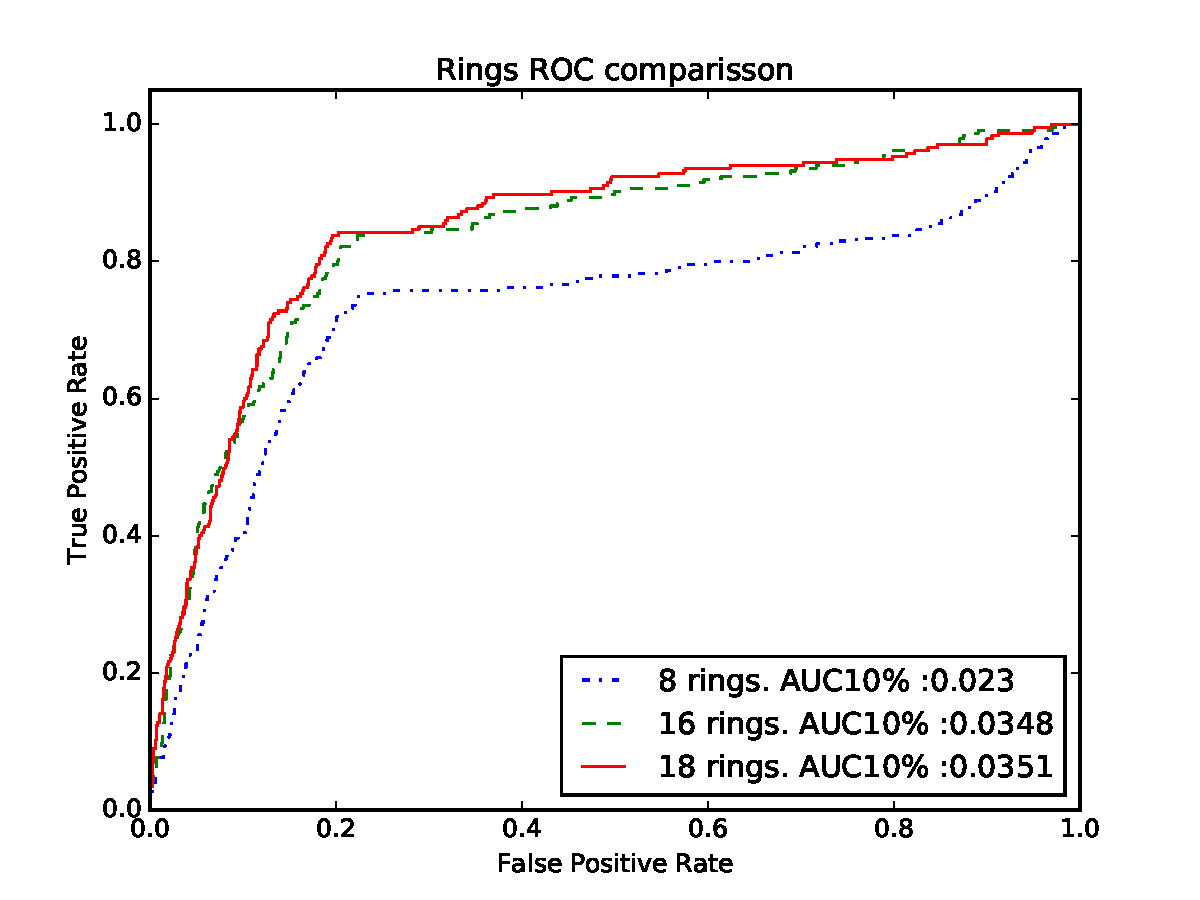
\includegraphics[width=0.8\textwidth]{results/ROC_rings}
\caption{Curvas ROC comparando classificadores SVM sob descritores de anéis com diferentes dimensões.}
\label{fig:roc-rings}
\end{figure}

Tendo visto que o classificador de 18 dimensões domina sob os outros na região de operação com menor TFP, decidiu-se selecionar esse descritor para seguir com a análise. Para tanto utilizou-se o conjunto de treinamento completo para o treinamento e posterior avaliação através do conjunto de teste, como visto nas tabelas \ref{cm:aneis18Tr} e \ref{cm:aneis18Te}.

\begin{table}
\cfmat{Anéis concêntricos com 18 dimensões, conjunto treinamento}{9890}{4}{79}{1143}{cm:aneis18Tr}
\cfmat{Anéis concêntricos com 18 dimensões, conjunto teste}{2564}{174}{158}{77}{cm:aneis18Te}
\end{table}

Outro descritor que também foi avaliado foi o de grades simples com dimensão 7x7, como demonstra as tabelas \ref{cm:gradesTr} e \ref{cm:gradesTe}.

\begin{table}
\cfmat{Grades simples, conjunto treinamento}{9881}{13}{36}{1186}{cm:gradesTr}
\cfmat{Grades simples, conjunto teste}{2445}{293}{181}{54}{cm:gradesTe}
\end{table}

\subsection{MLP}
Na estrutura MLP foram realizados testes com duas e três camadas intermediárias, com ativação RELU e um único perceptron de saída com ativação sigmoide indicando a probabilidade da amostra ser uma cabeça. Na configuração de duas camadas foram utilizados 512 e 256 perceptrons, respectivamente. Os resultados obtidos para o conjunto de treinamento são apresentados nas tabelas \ref{cm:MLP:Tr:5} e \ref{cm:MLP:Tr:9}. O resultado do conjunto de teste são apresentados nas tabela \ref{cm:MLP:Te:5} e \ref{cm:MLP:Te:9}.

\begin{table}
\cfmat{MLP, conjunto treinamento extendido $T=0.5$}{14533}{433}{104}{1828}{cm:MLP:Tr:5}
\cfmat{MLP, conjunto treinamento extendido $T=0.9$}{14794}{172}{252}{1680}{cm:MLP:Tr:9}

\cfmat{MLP, conjunto teste $T=0.5$}{2489}{249}{10}{225}{cm:MLP:Te:5}
\cfmat{MLP, conjunto teste $T=0.9$}{2635}{103}{25}{210}{cm:MLP:Te:9}
\end{table}

Para três camadas foram utilizados 1024, 512 e 256 perceptrons respectivamente, entretanto os resultados foram semelhantes aos obtidos com duas camadas, portanto o aumento em complexidade não é justificado visto que o desempenho permaneceu o mesmo.

\subsection{CNN}
Para redes convolucionais utilizou-se uma única camada convolucional RELU com 16 núcleos 3x3 seguida por max-pooling (3x3) e uma camada densamente conectada de 128 percepetrons RELU e finalmente saída única com ativação sigmoide. Essa topologia foi a que teve o melhor desempenho, obtendo 99\% de acurácia no conjunto de treinamento, demonstrados nas tabelas \ref{cm:CNN:Tr:5} e \ref{cm:CNN:Tr:9}. Também teve 96\% de acurácia no conjunto de teste, como observado nas tabelas \ref{cm:CNN:Te:5} e \ref{cm:CNN:Te:9}.

\begin{table}
\cfmat{CNN, $T=0.5$, conjunto treinamento extendido}{14934}{32}{23}{1909}{cm:CNN:Tr:5}
\cfmat{CNN, $T=0.9$, conjunto treinamento extendido}{14950}{16}{113}{1819}{cm:CNN:Tr:9}

\cfmat{CNN, $T=0.5$, conjunto de teste}{2521}{88}{16}{219}{cm:CNN:Te:5}
\cfmat{CNN, $T=0.9$, conjunto de teste}{2691}{47}{34}{201}{cm:CNN:Te:9}
\end{table}


\subsection{Discussão}
Verifica-se as curvas ROC dos classificadores correspondentes avaliados no conjunto de teste na figura \ref{fig:ROC}. Observando a região de interesse (TFP menor que 10\%) fica claro que os métodos profundos, com CNN e MLP, dominam os superficiais. Em mais detalhes, MLP domina entre TFP de 0.1\% a 1.3\%, a partir de onde CNN passa a dominar. Para especificar qual o melhor classificador entre os profundos é necessário saber exatamente a região de operação em que se deseja atuar. 

Observa-se que muitos classificadores obtiveram um desempenho elevado no conjunto de treinamento, em especial as redes convolucionais que obtiveram acurácia quase unitária (sob dataset balanceado) conforme tabelas \ref{cm:CNN:Tr:5} e \ref{cm:CNN:Tr:5}, demonstrando a alta capacidade do modelo. Nota-se, entretanto, que há grande discrepância entre o desempenho dos classificadores no conjunto de treinamento e de teste nos métodos superficiais, o que caracteriza \textit{overfitting}, como apontam as tabelas \ref{cm:aneis18Tr} e \ref{cm:aneis18Te}. Os métodos profundos, em contraste, apresentam uma boa generalização, como pode ser visto na tabela \ref{cm:CNN:Te:9}. Isso é explicado porque o modelo em questão foi corretamente especificado através no número de camadas e tamanho de filtros, de forma que sua capacidade se ajuste de forma adequada aos dados.

\begin{figure}
\centering
\begin{subfigure}{.5\textwidth}
  \centering
  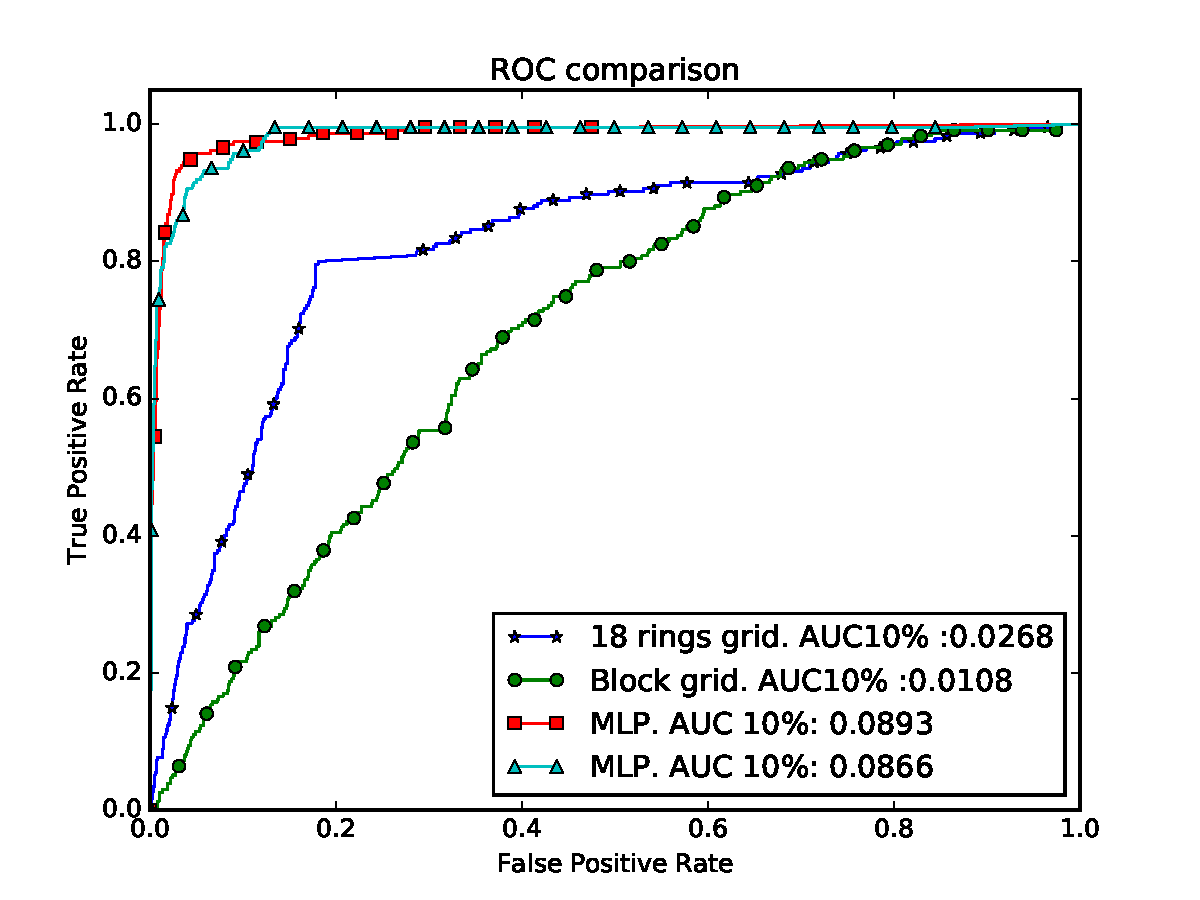
\includegraphics[width=\linewidth]{results/ROC_all}
\end{subfigure}%
\begin{subfigure}{.5\textwidth}
  \centering
  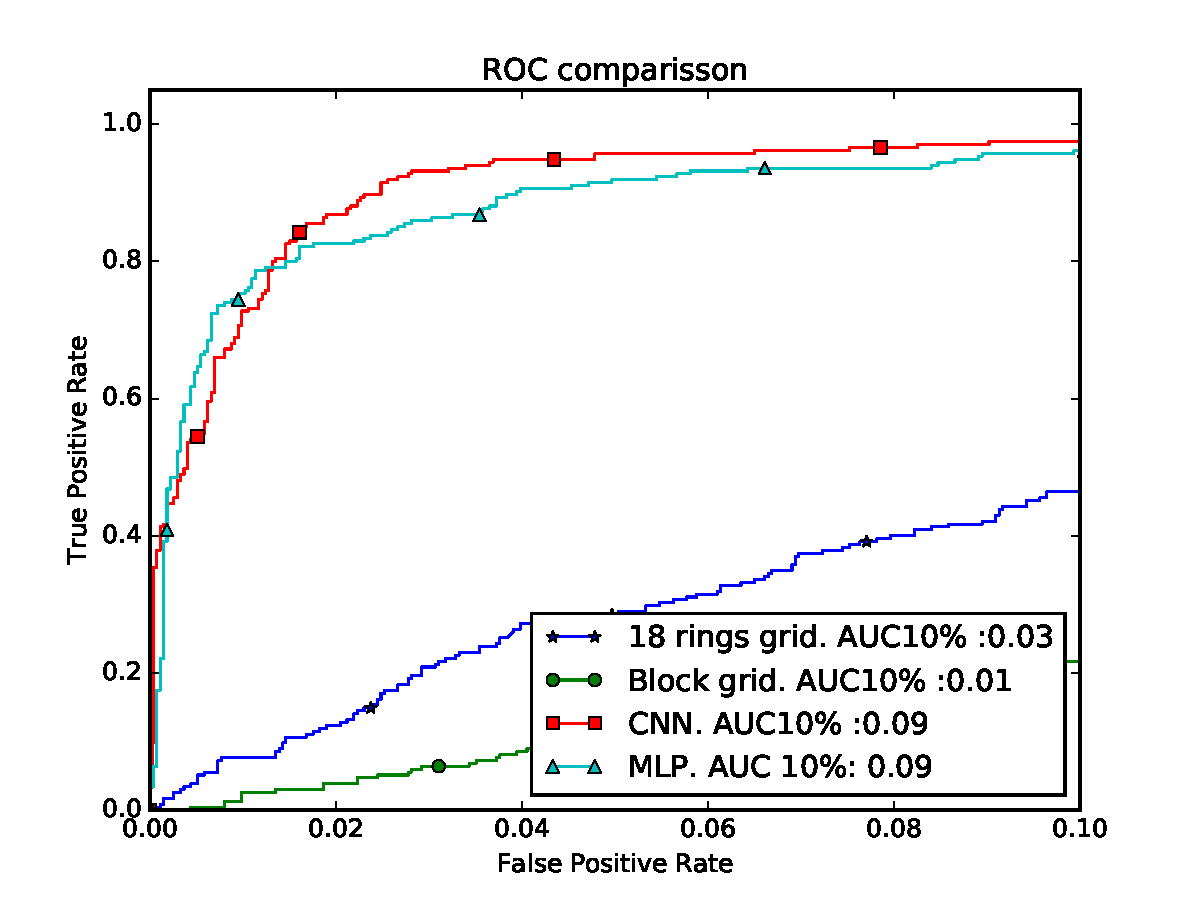
\includegraphics[width=\linewidth]{results/ROC_all_zoom}
\end{subfigure}
\caption{Curvas ROC comparando diferentes classificadores apresentados e zoom na região de interesse}
\label{fig:ROC}
\end{figure}

\section{Sistema completo}
Nessa seção serão comparados os resultados do sistema de extração de candidatos e de classificação como um todo. Tendo em vista os resultados da seção \ref{sec:resultados-classificadores}, a solução baseada na seleção de candidatos vista em \ref{sec:tradicional-candidatos} e classificador CNN apresentada no capítulo \ref{chap:class-profundo} será avaliada em detrimento das demais variações de classificadores. A última solução, cuja detecção e classificação são realizadas utilizando métodos profundos, vista no capítulo X também será avaliada.

	\chapter{Conclusão} \label{chap:conclusao}

Neste trabalho foi desenvolvido um sistema de detecção de pessoas em um ambiente indústrial cujo objetivo é interromper o funcionamento de equipamentos de transporte se uma pessoa for detectada, portanto, aumentar a segurança dos colaboradores na linha de produção. Duas propostas de implementação desse sistema foram avaliadas: a primeira baseada em métodos tradicionais de localização de objetos, vista no capítulo \ref{chap:tradicional}, e a segunda com uma abordagem híbrida, contando com classificadores profundos, vista no capítulo \ref{chap:class-profundo}. 

Cada solução apresenta suas especificidades e parâmetros, que precisam ser ajustados de maneira individual. O resultado apresentado no capítulo \ref{chap:resultados} demonstrou que o sistema com melhor performance foi que utilizou um classificador CNN. Esse fato corrobora uma tendência de avanço do uso das técnicas profundas, como já acontece em grandes competições acadêmicas.

Embora o sistema ainda não tenha sido implantado na indústria ainda, por desafios técnicos de montagem dos paineis de controle, os testes realizados utilizando vídeos de teste demonstram que o funcionamento do mesmo ocorre de maneira satisfatória. 

Das contribuições desse trabalho podem ser destacadas as comparações de classificadores superficiais (SVM) em conjunto com diferentes descritores aos classificadores profundos, nas diferentes topologias de rede CNN e MLP. O trabalho também demonstra que as técnicas profundas não se restringem a grandes conjuntos de dados (\textit{big data}), mas que pode ser empregado em situações com volume moderado de amostras, ainda que desbalanceadas.

Durante a implementação alguns desafios foram encontrados. Primeiramente na escolha dos descritores cuja escolha requer conhecimento específico da aplicação. Embora tenha sido utilizado o que recomenda a literatura e uma variação proposta nesse trabalho, os resultados não foram satisfatórios. Também houve dificuldade nas primeiras etapas de treinamento das redes profundas dado que o conjunto de treinamento era desbalanceado. Por fim, durante a fase de testes houve um conflito na unidade de processamento de vídeo que era utilizada simultâneamente pelo \textit{driver} da câmera stereo e pelo \textit{framework Keras}, mas que foi resolvido utilizando alocação de recursos da \textit{GPU}.

\section*{Trabalhos futuros}

Os vídeos utilizados para gerar o dataset desse trabalho só puderam ser gravados em uma ocasião. Isso proporcionou um conjunto de dados moderadamente limitado no sentido de ser desbalanceado e ter um padrão de peças que seriam encontradas na produção. É possível que após a instalação do sistema na fábrica ocorram mais falsos positivos do que previsto no vídeo de teste, justamente pela mudança no padrão de peças.

Pode-se resolver esse problema gravando todas as amostras classificadas como positivas e manualmente selecionando as que foram falsos positivos. Numa próxima etapa pode-se fazer um treinamento de ajuste, variando parâmetros apenas das últimas camadas, responsáveis pela classificação de maneira a ter uma melhor performance real.

Tendo em vista o grande potencial das técnicas de aprendizado profundo, tanto os resultados aqui apresentados como os do estado da arte, idealizou-se uma terceira solução integralmente baseado em estruturas profundas. Nesta proposta não existe seleção de candidatos: o quadro inteiro é tido como entrada do classificador, que deve então retornar uma saída indicando a existência ou não de pessoas na cena.

A topologia de rede proposta é convolucional com uma saída bidimensional que representa um mapa de probabilidades de existir uma cabeça em cada posição deste mapa. Essa topologia permite maior generalização do problema de forma que haja invariância à translação das cabeças no quadro. Além disso, essa saída em mapa permite que a rede seja treinada mais facilmente se comparada à uma única saída que representa a probabilidade do quadro conter cabeça. Isso advém do fato de uma única saída não permitir especificar qual é o objeto de interesse, portanto o treinamento irá exigir um número muito maior de amostras até conseguir modelar esse conhecimento.

Por limitação de tempo essa solução não pôde ser implementada até a apresentação desse trabalho, porém deve seguir em desenvolvimento.


	\begin{frame}[standout]
	  Dúvidas?
	\end{frame}

	\begin{frame}[standout]
	  Obrigado pela atenção!
	\end{frame}

\end{document}
